\input{glyphtounicode}
\pdfgentounicode=1
\documentclass[conference,letterpaper]{IEEEtran}
\IEEEoverridecommandlockouts
\usepackage{cmap}
\usepackage[T1]{fontenc}
\usepackage{amsmath,amssymb,graphicx,booktabs,multirow,array,url,cite,balance,float}
\usepackage[bookmarks=false,hidelinks]{hyperref}
\urlstyle{same}
\setcounter{topnumber}{1}\setcounter{totalnumber}{4}
\setlength{\textfloatsep}{6pt plus 4pt minus 1pt}
\setlength{\floatsep}{6pt plus 2pt minus 1pt}
\setlength{\intextsep}{6pt plus 2pt minus 1pt}
% Set before maketitle so IEEEtran computes the title spacing consistently.
\setlength{\dbltextfloatsep}{6pt plus 4pt minus 1pt}
\title{Selective Recovery for Multilingual ASR:\\Candidate Acquisition and Acceptance}
\author{
\IEEEauthorblockN{Zhifan Pan\textsuperscript{1,2,3}, Maihemuti Maimaiti\textsuperscript{1,2,3,$*$},
Yingxiong Gao\textsuperscript{1,2,3},
Yuhui Ming\textsuperscript{1,2,3}, Aishan Wumaier\textsuperscript{1,2,3}}
\IEEEauthorblockA{\textsuperscript{1}School of Computer Science and Technology, Xinjiang University, Urumqi, China\\
\textsuperscript{2}Xinjiang Multimodal Intelligent Processing and Information Security\\
Engineering Technology Research Center, Xinjiang University, Urumqi, China\\
\textsuperscript{3}Joint International Research Laboratory of Silk Road Multilingual\\
Cognitive Computing, Xinjiang University, Urumqi, China\\
\textsuperscript{$*$}Corresponding author: \texttt{mahmutjan@xju.edu.cn}}
}

\begin{document}\maketitle\flushbottom
% Modest elastic paragraph spacing keeps short columns from stretching headings alone.
\setlength{\parskip}{0pt plus 4pt}
\begin{abstract}
Fallback recovery depends on both candidate acquisition and acceptance. We isolate these decisions using a text-compression trigger and fixed four-feature selector. On 7,500 frozen Common Voice recordings, selective recovery lowers macro word error rate by 2.26 percentage points and matches unconditional recovery's error counts in all three seeds. Development-exposed CV27 TEST retains 99.98\% of pooled positive edit gain. Matched-bank unweighted ranking trails expected risk in every seed; Direct's and edit-weighted ranking's advantages concentrate in individual checkpoints and depend on source. Three-checkpoint stratified timing estimates show up to 5.15\% savings over unconditional reranked recovery; Native remains faster. Code: \url{https://github.com/Zhifan-Pan/ISCAS2027}.
\end{abstract}
\begin{IEEEkeywords}
multilingual speech recognition, selective recovery, candidate acquisition, N-best reranking, confidence estimation, conditional computation
\end{IEEEkeywords}

\section{Introduction}
Acquisition may preserve corrections under one selector but discard them under another. We separate acquisition from acceptance to study this dependence.

Multilingual N-best reranking~\cite{gaur2022,yan2025wild}, discriminative rescoring~\cite{rescorebert,discriminative2023,audioattention2019}, voting~\cite{fiscus1997} and confusion networks~\cite{mangu2000} exploit existing hypotheses. Generative correction expands banks~\cite{kuo2026framework,dutta2022,progres2024,whisperingllama}; risk-based pruning and ASR sampling allocate computation~\cite{cheng2023pruning,jinnai2025mbrasr}.

Conditional computation uses recognizer cascades~\cite{xue2025sima}, selective passes~\cite{aleksic2025}, encoder proxies~\cite{fathullah2024proxies}, selective correction~\cite{lim2025hybrid} or language-specific distillation~\cite{ferraz2024distil}. Confidence need not predict computational benefit~\cite{jitkrittum2023cascade}: acceptance determines which acquired hypotheses improve output.

With recognizer and language labels frozen, we compare acquisition within sources. A frozen panel evaluates the original policy; retrospective controls assess acceptance objectives~\cite{mwer2018,ranknet2005,goel2000mbr} and acquisition budgets.

\begin{figure*}[t]\centering
% The vector PDF supplies its own transparency group; do not inject a duplicate.
\makeatletter
\ifdefined\Gread@transgroupfalse
\let\Gread@transgrouptrue\Gread@transgroupfalse
\fi
\makeatother
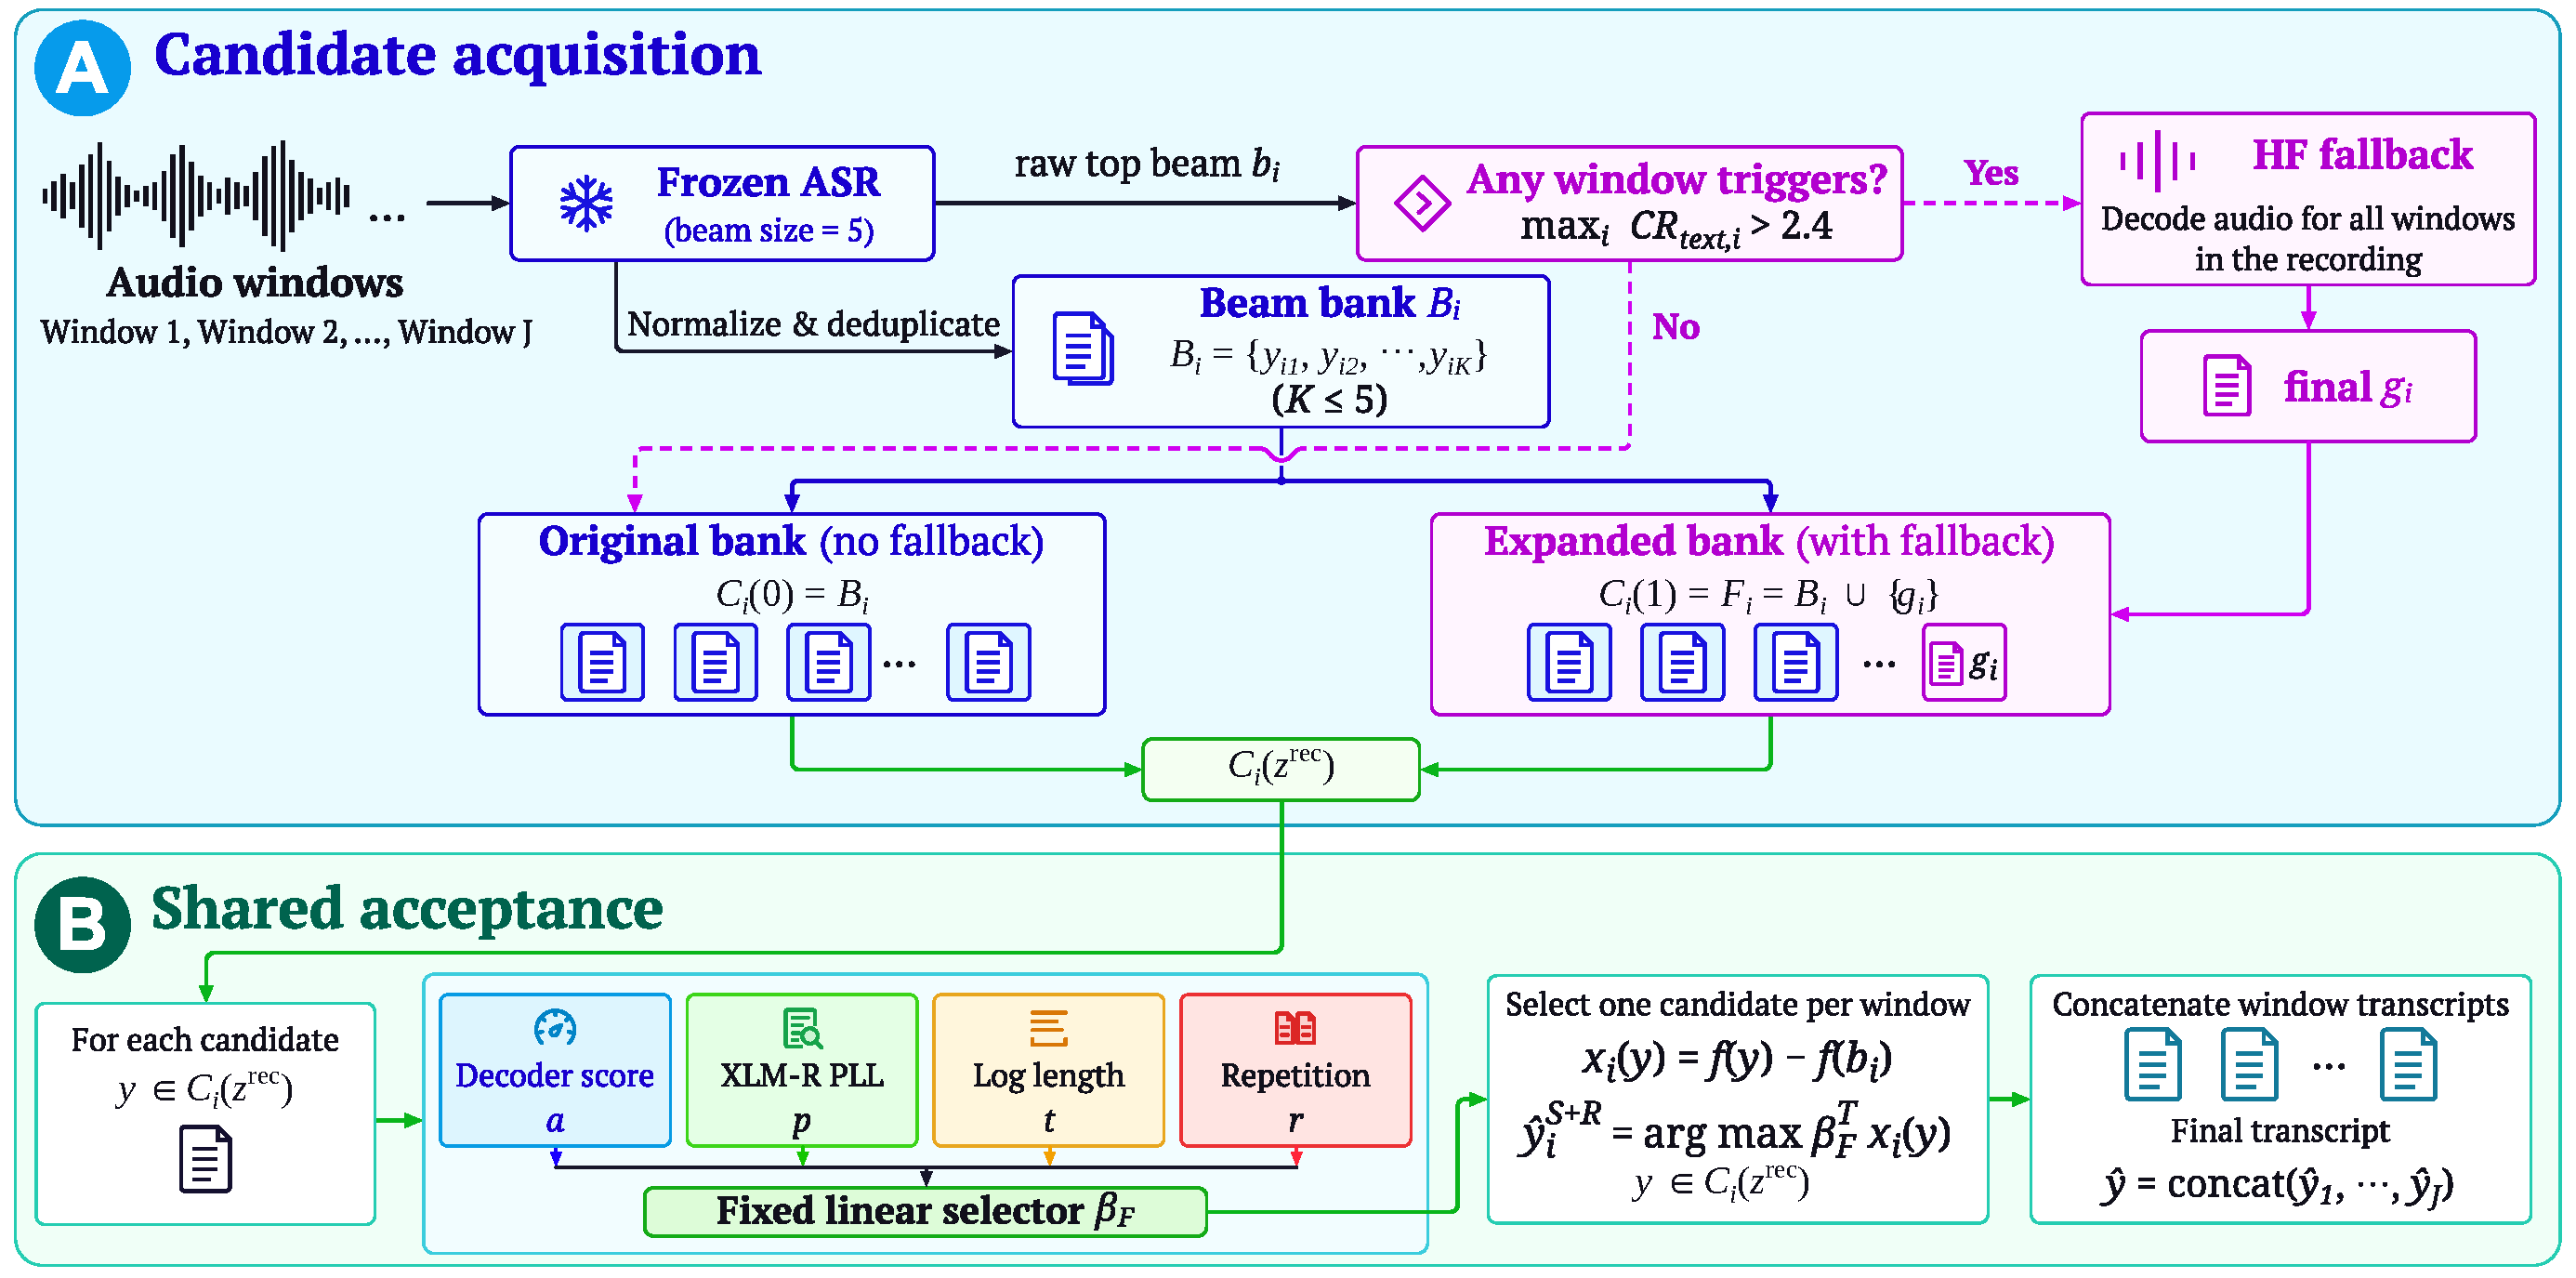
\includegraphics[width=0.80\textwidth]{figures/Figure1_Vector.pdf}
\caption{Acquisition (A) expands every window's candidate bank if any window triggers. Acceptance (B) applies the same fixed four-feature selector to the original or expanded bank. Selected window transcripts are then concatenated.}
\label{fig:workflow}\end{figure*}

\section{Controlled Acquisition and Acceptance}
\subsection{Recording-level acquisition}
Normalizing and deduplicating five beams per window $i$ gives $B_i$, retaining first occurrences and sources; $b_i$ is the raw top beam. Fallback $g_i$ gives $F_i=B_i\cup\{g_i\}$, at most six candidates. The outer $\mathrm{CR}_{\mathrm{text}}$ divides top-beam UTF-8 byte length by zlib-compressed length, or is zero for empty bytes. With $z_i=\mathbf1\{\mathrm{CR}_{\mathrm{text},i}>2.4\}$ and $z^{\mathrm{rec}}=\max_i z_i$, any trigger acquires fallback for every window, including singletons.

Recovery uses final Hugging Face fallback at temperatures $0,0.2,\ldots,1$, with compression, log-probability and no-speech thresholds $1.35$, $-1$ and $0.6$. Internal compression uses serialized token-ID bytes, unlike the outer text scale. Transformers v4.57.6 lists $1.35$ as common~\cite{hfwhisper4576}. Native HF uses the same configuration. Retries are conditional; intermediate hypotheses never enter the bank.

\subsection{Four-feature Shared acceptance}
For $f(y)=(a,p,t,r)$, decoder score $a$ averages teacher-forced log probabilities over $T$ body tokens, excluding prefix, padding and end tokens; $t=\log(1+T)$. XLM-R-base pseudo-log-likelihood $p$~\cite{xlmr,mlmscoring}, or PLL, averages log probabilities of individually masked nonspecial subwords in the original string, using centered windows of at most 510 subwords rather than within-word masking~\cite{kauf2023}. No body tokens gives $a=t=0$; no PLL targets gives $p=0$. Normalization-only emptiness need not give zero features.

For normalized words $w_{1:M}$, define the overlapping $n$-gram count $c_y(u)=\sum_{k=1}^{M-n+1}\mathbf1\{w_{k:k+n-1}=u\}$. Repetition is
\begin{equation}
r_{n,h}(y)=\frac{\sum_{j=1}^{M-n+1}\mathbf1\{c_y(w_{j:j+n-1})\ge h\}}{\max(1,M-n+1)}.
\label{eq:repetition}
\end{equation}
We use $r=r_{4,3}$, which is zero for $M<4$. Repetition is also a target of unlikelihood training~\cite{welleck2020}.

Centering $x_i(y)=f(y)-f(b_i)$ preserves rankings and softmax probabilities. Feature-wise RMS scales $s\in\mathbb R^4_{>0}$ use training-fold pairs $\{(i,k):i\in\bigcup_{\ell=1}^L\mathcal I_\ell,\ y_{ik}\in C_i\setminus\{b_i\}\}$ in fitting banks $C_i$; scales below $10^{-12}$ become one. With edit benefit $\Delta_{ik}=E(b_i,y_i^*)-E(y_{ik},y_i^*)$ and $\pi_{ik}=\operatorname{softmax}_k\!\left(\theta^\top\operatorname{diag}(s)^{-1}x_{ik}\right)$, expected-risk fitting~\cite{mwer2018} minimizes
\begin{equation}
\mathcal L(\theta)=-\frac1L\sum_{\ell=1}^L\frac{\sum_{i\in\mathcal I_\ell}\sum_k\pi_{ik}\Delta_{ik}}{N_\ell}+\lambda\|\theta\|_2^2.
\label{eq:risk}
\end{equation}
Here $\mathcal I_\ell=\{i:\operatorname{lang}(i)=\ell\}$ indexes fitting windows, $N_\ell$ counts reference words and $L=5$.
\par
Shared weights $\beta_F=\operatorname{diag}(s)^{-1}\theta$ are fitted per run on greedy-expanded DEV and fixed across sources, with bank-order ties. Let $\hat{y}_i^B=\arg\max_{y\in B_i}\beta_F^\top x_i(y)$, $C_i(0)=B_i$ and $C_i(1)=F_i$. Then
\begin{equation}
\begin{aligned}
\hat{y}_i^{S+R}&=\arg\max_{y\in C_i(z^{\mathrm{rec}})}\beta_F^\top x_i(y),\\
\hat{y}_i^{\mathrm{Direct}}&=\begin{cases}\hat{y}_i^B,&z^{\mathrm{rec}}=0,\\g_i,&z^{\mathrm{rec}}=1.\end{cases}
\end{aligned}\label{eq:accept}
\end{equation}
B reranks $B_i$; N+R requests and reranks $F_i$ unconditionally. Direct bypasses selection and PLL on triggers, retaining B elsewhere. CV27 has $z^{\mathrm{rec}}=z_i$; multi-window FLEURS uses the recording flag. Concatenated transcripts receive complete-reference scoring. Shared fixes acceptance to isolate acquisition.

\subsection{Matched acceptance controls}
G4 is the original $\beta_F$. H4 refits expected risk on complete HF-expanded DEV banks; H3 uses the same objective with $(a,t,r)$. HR4 fits RankNet~\cite{ranknet2005} on H4's banks and four features. Its logistic loss favors lower-edit candidates in unequal-edit pairs, with language-reference normalization and equal total bank weight. HWR4 additionally weights pairs by $|E_j-E_k|/c$, where $c$ is the training-fold mean edit gap under the original pair weights.

Five component folds group clients and reference texts within languages. RMS uses training folds; held-fold hard macro WER chooses among 49 log-spaced penalties from $10^{-4}$ to $1$, favoring stronger regularization on ties. Full-DEV fitting uses zero-initialized L-BFGS-B. Singletons retain errors and reference denominators but contribute no ranking pairs.

Same-bank minimum Bayes risk (MBR)~\cite{goel2000mbr} minimizes expected word edits. U-MBR is uniform; D-MBR uses body scores $\operatorname{softmax}(Ta/\tau)$, not calibrated sequence posteriors. DEV WER selects $\tau\in\{0.1,0.3,1,3,10\}$, favoring larger values on ties. Candidate ties retain bank order.

A \emph{complete policy} uses its acceptor on both banks. A \emph{triggered-subset evaluation} changes acceptance only on triggers, retaining G4 elsewhere and full-panel denominators. H3Direct uses H3 off-trigger and final HF on-trigger.

\section{Data and Evaluation}
We adapt Whisper-small~\cite{whisper} on 44.60\,h of FLEURS TRAIN~\cite{fleurs} to Arabic, Persian, Polish, Turkish and Italian using LoRA~\cite{lora} with three different random seeds: 4,656 updates each, rank and scale four, zero dropout, all attention projections. Adaptation excludes CV27 TRAIN; reported fits exclude FLEURS DEV. Selectors and gates use CV27 DEV. Complete TEST has 3,665 FLEURS and 58,514 Common Voice 27.0 recordings~\cite{cv2020} from release \texttt{2026-09-11}. TEST informed development, making comparisons retrospective.

Confirmation uses 7,500 CV27 TRAIN recordings, 1,500 per language, excluding previously accessed recordings, audio and reference texts. Predictions, stopping rules and the 0.10\,pp one-sided noninferiority margin were locked before reference evaluation under procedural controls. Within-panel correlation is addressed by 10,000 synchronized within-language speaker-component bootstrap draws. Recurring Common Voice speakers across splits restrict generalization to the observed speaker-clustered sampling frame. Later gates, refits and window policies remain retrospective.

Decoding uses known languages, bfloat16, five beams, length penalty one, native suppression and a 444-token cap in Transformers 4.57.6. At 16\,kHz, $N$ samples yield $J=\lceil N/480000\rceil$ windows bounded by $\lfloor jN/J\rfloor$, without previous-window text conditioning.
Deduplication, WER and $r$ share NFC normalization, digit unification, punctuation-to-space, Persian mapping and Turkish casing~\cite{normalization}. Source RNG mappings stay fixed.

\begin{samepage}
WER aggregates within languages before averaging five languages and three seeds; calls pool seed--recordings. Seed diagnostics use consistent order. TEST intervals use 2,000 paired language-internal client/reference-component draws, synchronized across seeds and conditional on frozen fits and source draws. FLEURS controls are descriptive because component metadata are unverified.\par
\end{samepage}

Costs use 255 FLEURS and 472 CV27 recordings: all first-checkpoint triggers or Native-output changes plus ten ordinary recordings per language--duration-quintile cell, weighted by inclusion probability. Unsampled later-checkpoint triggers number five on FLEURS and 207 on CV27, or 0.05\% and 0.12\% of seed--recordings in probability-sampled strata. Triggered N+R and S+R perform identical acquisition and scoring operations. Both studies use three randomized paired A40 rounds, resident models, encoder/first-search reuse and 32-mask PLL batches. Synchronized waveform-to-output timing excludes loading, warmup and interfered blocks. Session-conditional intervals use 4,000 paired stratified bootstrap draws with finite-population correction and equal checkpoint weights synchronized in A.

\section{Results}
\subsection{Acquisition with fixed acceptance}
\begin{table}[H]\centering\footnotesize
\caption{WER (\%); pp gains and contrasts computed before rounding. Checks: HF acquisition, CR gate, R reselection; $\dagger$: R off-trigger.}\label{tab:paths}
\setlength{\tabcolsep}{3pt}\renewcommand{\arraystretch}{1.00}
\begin{tabular}{@{}lccclrr@{}}\toprule
Path & HF & CR & R & Scorer & FLEURS & CV27\\\midrule
Raw beam-5 top-1 & -- & -- & -- & -- & 18.90 & 36.41\\
Native HF & $\checkmark$ & -- & -- & -- & 18.55 & 33.80\\
B & -- & -- & $\checkmark$ & G4 & 17.45 & 33.98\\
N+R & $\checkmark$ & -- & $\checkmark$ & G4 & 17.09 & 31.68\\
S+R & $\checkmark$ & $\checkmark$ & $\checkmark$ & G4 & 17.09 & 31.68\\
Direct & $\checkmark$ & $\checkmark$ & $\checkmark^{\dagger}$ & G4 & 17.09 & 31.46\\
H3Direct & $\checkmark$ & $\checkmark$ & $\checkmark^{\dagger}$ & H3 & 18.68 & 33.64\\
\midrule\multicolumn{7}{c}{Reference-assisted lower bounds on TEST}\\
\multicolumn{5}{l}{Original-bank oracle} & 16.19 & 30.19\\
\multicolumn{5}{l}{Full-HF oracle} & 15.83 & 27.68\\
\multicolumn{5}{l}{CR-routed oracle} & 15.83 & 27.68\\
\multicolumn{5}{l}{S+R gap to routed oracle, pp} & 1.26 & 4.00\\
\midrule\multicolumn{7}{c}{Frozen CV27 confirmation: 7,500 recordings}\\
\multicolumn{4}{l}{} & B & N+R = S+R & Gain\\\midrule
\multicolumn{4}{l}{Macro-average} & 35.02 & 32.75 & 2.26\\
\midrule\multicolumn{5}{l}{Contrast} & $\Delta$WER & 95\% upper bound\\
\multicolumn{5}{l}{S+R $-$ B} & -2.26 & -1.32\\
\multicolumn{5}{l}{S+R $-$ N+R} & 0.00 & 0.00\\
\bottomrule\end{tabular}\end{table}

Frozen-panel S+R gains 2.26\,pp over B: 2.04, 0.20 and 4.54\,pp by seed. Substitution, deletion and insertion counts match N+R in every seed, meeting the prespecified 0.10\,pp margin. Among 61 triggers, 49 improve and two worsen edits versus B. The zero-loss interval remains panel-specific.

Post-lock Direct has 32.71\% WER and S+R 32.75\%; both beat B and Native's 34.87\% by over 2.1\,pp. From unrounded means, Direct minus S+R is $-0.05$\,pp, with retrospective paired speaker-bootstrap 95\% CI [$-0.19$, $+0.04$].\par
\begin{samepage}
The frozen archive locked G4 scores and transcripts to isolate acquisition; refits use full TEST.\par
\end{samepage}

TEST Shared retains 99.98\% of CV27 positive edit gain with full-language denominators. FLEURS retains all 10 beneficial instances at 0.09\% calls; CV27 retains 370 of 373 at 0.30\%, missing five edits. N+R and S+R outputs differ after normalization on one FLEURS and 13 CV27 nontriggers despite nearly identical WER.

Reference-assisted oracles minimize full-reference edits over original, expanded or CR-routed banks, including concatenated two-window candidates. Routing changes the bound by under 0.01\,pp; CV27 S+R remains 4.00\,pp above it. Top-1 to B measures reselection, not PLL alone.

\subsection{Acceptance changes recovery opportunities}
Bypassing the greedy-trained selector on triggers, Direct lowers CV27 WER while retaining 67.13\% of its own positive edit gain, against Shared's 99.98\%. Relative to unconditional final HF, it forgoes 1.24\,pp of beneficial changes but avoids 3.58\,pp of harmful changes.

Shared beats Direct by 0.53\,pp for greedy recovery and 0.43\,pp for one $T=0.2$ draw. HF reverses this ranking by 0.22\,pp, with 95\% CI [0.11, 0.37]. Direct-minus-Shared differences of $-0.68$, $+0.00$ and $+0.02$\,pp by seed concentrate the advantage in one checkpoint. DEV favored HF reselection at 30.08\% versus 30.09\%, motivating fixed acceptance.

\subsection{Acceptance on matched HF banks}
\begin{table}[!t]\centering\footnotesize
\caption{Same-HF TEST WER (\%); gain B$-$S (pp) before rounding. Checks: PLL, pairwise P, edit-gap weighting W.}\label{tab:hfacceptors}
\setlength{\tabcolsep}{2pt}\renewcommand{\arraystretch}{1.00}
\begin{tabular}{@{}lcccrrrrrr@{}}\toprule
 & & & & \multicolumn{3}{c}{FLEURS} & \multicolumn{3}{c}{CV27}\\
\cmidrule(lr){5-7}\cmidrule(lr){8-10}
Acceptor & PLL & P & W & B & S & Gain & B & S & Gain\\\midrule
G4 & $\checkmark$ & -- & -- & 17.45 & 17.09 & 0.37 & 33.98 & 31.68 & 2.30\\
H4 & $\checkmark$ & -- & -- & 17.46 & 17.09 & 0.37 & 33.97 & 31.52 & 2.45\\
HR4 & $\checkmark$ & $\checkmark$ & -- & 17.51 & 17.14 & 0.37 & 34.02 & 32.30 & 1.72\\
H3 & -- & -- & -- & 19.05 & 18.68 & 0.37 & 36.15 & 33.77 & 2.38\\
HWR4 & $\checkmark$ & $\checkmark$ & $\checkmark$ & 17.47 & 17.10 & 0.37 & 33.97 & 31.44 & 2.53\\
U-MBR & -- & -- & -- & 19.14 & 19.14 & 0.00 & 36.91 & 36.88 & 0.03\\
D-MBR & -- & -- & -- & 18.92 & 18.75 & 0.17 & 36.09 & 34.48 & 1.60\\
\midrule\multicolumn{10}{c}{CV27 $\Delta$WER [individual 97.5\% CI]: original family}\\
\multicolumn{7}{l}{Triggered HR4 $-$ H4} & +0.72 & \multicolumn{2}{c}{[+0.40, +1.16]}\\
\multicolumn{7}{l}{Complete H3 $-$ H4} & +2.25 & \multicolumn{2}{c}{[+2.16, +2.34]}\\
\multicolumn{10}{l}{Later two-comparison family}\\
\multicolumn{7}{l}{Triggered U-MBR $-$ H4} & +2.51 & \multicolumn{2}{c}{[+1.93, +3.18]}\\
\multicolumn{7}{l}{Triggered HWR4 $-$ H4} & -0.08 & \multicolumn{2}{c}{[-0.15, -0.03]}\\
\bottomrule\end{tabular}\end{table}

With the same four-feature architecture, HWR4 achieves the lowest complete CV27 WER, 31.44\%, against Direct's 31.46\%. Triggered HR4 minus H4 is positive in every seed: $+0.91$, $+0.08$ and $+1.17$\,pp. Edit-gap weighting reverses the mean to $-0.08$\,pp, concentrated in one checkpoint: $0.00$, $-0.25$ and $+0.01$\,pp for HWR4 minus H4.

FLEURS gains round to 0.37\,pp for all five acceptors: off-trigger S equals its own B; on one of ten triggers, H3's B has two fewer errors while S error counts match. Language and checkpoint averaging reduces this gain difference below 0.006\,pp.

\begin{samepage}
Table~\ref{tab:hfacceptors} gives 95\% Bonferroni coverage per family; the later family uses 10,000 synchronized draws.\par
\end{samepage}

The MBR controls also trail H4~\cite{jinnai2025mbrasr}. H3-based policies trail H4 and Direct despite baseline gains. Nontriggers account for 97.23\% of the refitted H3--H4 gap, measuring neither PLL causality nor time share.

\subsection{Cost, heterogeneity and supporting diagnostics}
\begin{table}[!t]\centering\footnotesize
\caption{Population-weighted mean ms; observed peak allocated MiB with both models resident. Three paired rounds per study.}\label{tab:cost}
\setlength{\tabcolsep}{4pt}\renewcommand{\arraystretch}{1.00}
\begin{tabular}{@{}lrrrr@{}}\toprule
 & \multicolumn{2}{c}{FLEURS} & \multicolumn{2}{c}{CV27}\\
Path & ms & MiB & ms & MiB\\\midrule
\multicolumn{5}{c}{A: Four paths, three checkpoints}\\
Native HF & 1291.7 & 2980.8 & 517.4 & 2813.8\\
B & 1352.7 & 3144.9 & 591.9 & 3133.1\\
N+R & 1436.8 & 2988.3 & 639.2 & 3133.1\\
S+R & 1362.8 & 3189.7 & 610.0 & 3133.1\\
\midrule
\multicolumn{5}{c}{B: Seven paths, one checkpoint}\\
Native HF & 1304.8 & 2978.4 & 531.2 & 2811.8\\
Raw top-1 & 1222.6 & 2946.6 & 479.9 & 2571.0\\
B & 1364.0 & 3142.4 & 605.1 & 3131.1\\
N+R & 1449.6 & 2986.3 & 657.9 & 3131.1\\
S+R & 1374.5 & 3187.2 & 628.0 & 3131.1\\
Direct & 1372.8 & 3187.2 & 625.8 & 2811.8\\
H3Direct & 1314.0 & 3187.2 & 586.4 & 2811.8\\
\midrule
\multicolumn{5}{c}{S+R saving versus N+R: \% [pointwise 95\% CI]}\\
A & \multicolumn{2}{c}{5.15 [2.84, 9.41]} & \multicolumn{2}{c}{4.57 [4.40, 4.73]}\\
B & \multicolumn{2}{c}{5.18 [2.88, 9.39]} & \multicolumn{2}{c}{4.54 [4.44, 4.66]}\\
\midrule
\multicolumn{5}{c}{Within-study B strategy differences, not stage times}\\
B $-$ Raw top-1, ms & \multicolumn{2}{c}{141.4} & \multicolumn{2}{c}{125.2}\\
N+R $-$ B, ms & \multicolumn{2}{c}{85.6} & \multicolumn{2}{c}{52.8}\\
S+R $-$ B, ms & \multicolumn{2}{c}{10.5} & \multicolumn{2}{c}{22.9}\\
Increment saved & \multicolumn{2}{c}{87.7\%} & \multicolumn{2}{c}{56.6\%}\\
\bottomrule\end{tabular}\end{table}

For systems using B, S+R preserves N+R's accuracy gain while reducing recovery overhead; Native and B remain faster. Study B's weighted B-minus-Raw increments are 141.4\,ms on FLEURS and 125.2\,ms on CV27; S+R saves 87.7\% and 56.6\% of their N+R increments over B (Table~\ref{tab:cost}). In 25 unweighted CV27 recordings, teacher scoring averages 85.9\,ms and PLL 149.3\,ms; two singletons skip both. These profile means describe a subset; strategy increments weight all strata.

Study B's Raw top-1 and H3Direct skip PLL. H3Direct saves 6.29\% versus Direct but trails Native by 55.2\,ms on CV27, with 95\% CI [52.3, 58.2]; FLEURS' interval spans zero. H4 and HWR4 change G4's coefficients within the same four-feature scoring architecture; Table~\ref{tab:cost} measures the listed paths. Trigger-selective PLL remains a future optimization.

\begin{table}[t]\centering\footnotesize
\caption{TEST gain: seed mean; calls: pooled seed--recordings.}\label{tab:language}
\setlength{\tabcolsep}{5pt}\renewcommand{\arraystretch}{1.00}
\begin{tabular}{@{}lrrrr@{}}\toprule
 & \multicolumn{2}{c}{FLEURS} & \multicolumn{2}{c}{CV27}\\
Language & Gain, pp & Calls, \% & Gain, pp & Calls, \%\\\midrule
Arabic & 0.64 & 0.23 & 1.40 & 0.11\\
Persian & 1.20 & 0.27 & 9.05 & 1.15\\
Polish & 0.00 & 0.00 & 0.30 & 0.33\\
Turkish & 0.00 & 0.00 & 0.51 & 0.03\\
Italian & 0.00 & 0.00 & 0.23 & 0.02\\
\midrule\multicolumn{5}{c}{Empty-HF acceptance: 18 instances, 11 CV27 recordings}\\
\multicolumn{2}{l}{Acceptance minus B reversion} & $S:-118$ & $D:+120$ & $I:-1995$\\
\bottomrule\end{tabular}\end{table}

Empty TEST candidates enter only through HF fallback, with $f(\emptyset)=(0,0,0,0)$ and centered score $\beta_F^\top x_i(\emptyset)=-\beta_F^\top f(b_i)$. The margin $-\beta_F^\top f(y)>0$ holds under signs $(+,+,-,-)$ when $a,p\le0$, $t>0$ and $r\ge0$, even at $r=0$. Centering preserves this preference, not a transcript probability.

Reverting all 18 empty HF acceptances in 11 CV27 recordings to B gives a deterministic nonempty guard. It retains 91.52\% of CV27 gain: 2.10\,pp at 31.88\% WER.\par
\begin{samepage}
The insertion--deletion tradeoff (Table~\ref{tab:language}) is consistent with hallucination suppression~\cite{baranski2025nonspeech}; acoustic interpretation requires silence labels.\par
\end{samepage}

\begin{samepage}
H4+$e$ refits with $e(y)=\mathbf1\{y=\emptyset\}$ on H4's DEV folds and grid. With one or two DEV empties per checkpoint, it matches H4's rounded 31.52\% CV27 WER and retains all 18 empty acceptances.\par
\end{samepage}

Persian supplies 78.77\% of CV27 TEST gain, with 9.05\,pp at 1.15\% calls, and 84.07\% of confirmation gain. Polish, Turkish and Italian have zero FLEURS calls and gains. Script, noise and LoRA effects remain coupled (Table~\ref{tab:language}).

FLEURS' 22 two-window recordings yield 52.69\% of net gain. Cached full-TEST local Shared preserves counts, cutting requests from 15 to 10: four to two, three to two and eight to six by seed. Local Direct changes WER by under 0.01\,pp; live RNG may differ.

Bulgarian and Croatian greedy WER stays at 37.51\%. The earlier 4,431-recording panel gives S+R-minus-B of $-0.08$\,pp, with 95\% CI [$-0.23$, $0.00$]. SeamlessM4T~\cite{seamless2023,seamlessv1nature} greedy CV27 WER falls from 12.96\% to 12.69\% at 0.08\% calls. DEV-tuned MBR reaches 12.55\% against risk's 12.66\% on greedy-expanded banks; full HF remains unvalidated.

HF12 ridge regression predicts fixed-G4 edit gain on grouped CV27 DEV folds from twelve pre-acquisition features: $\log(1+d)$ for duration $d$ in seconds, $\log(1+|B_i|)$, top-two decoder-score gap, softmax-$a$ entropy, population standard deviation and range of $a$, mean $|a-a(b_i)|$, ranges of $t$ and $r$, top-beam $\mathrm{CR}_{\mathrm{text}}$ and $r(b_i)$, and maximum repetition. Conditional on G4's fit, predicted negative gain below DEV's $q=3\times10^{-3}$ quantile triggers multi-candidate windows. HF12 and CR yield 31.71\% WER at 0.29\% and 0.26\% CV27 calls. Their interval spans zero without establishing equivalence; equal-call ranking favors HF12. FLEURS calls are 178, two and five by seed.

\section{Conclusion}
Sparse acquisition matches unconditional recovery across three frozen-panel seeds and reduces reranked-pipeline latency. Expected risk consistently beats unweighted ranking; Direct and edit-weighted ranking depend on checkpoint and source.
\section*{Acknowledgment}
Supported by the National Natural Science Foundation of China under Grant 62466058 and Autonomous Region Key R\&D Program under Grant 2025B03042-1.
\label{iscas:body-end}\clearpage\raggedbottom\balance
\label{iscas:references-start}
% IEEEtran bibliography style; verified entries manually maintained.
\begin{thebibliography}{99}
% Keep each bibliographic entry intact when balancing the final two columns.
\interlinepenalty=10000
\providecommand{\url}[1]{#1}
\csname url@samestyle\endcsname
\providecommand{\newblock}{\relax}
\providecommand{\bibinfo}[2]{#2}
\providecommand{\BIBentrySTDinterwordspacing}{\spaceskip=0pt\relax}
\providecommand{\BIBentryALTinterwordstretchfactor}{4}
\providecommand{\BIBentryALTinterwordspacing}{\spaceskip=\fontdimen2\font plus
\BIBentryALTinterwordstretchfactor\fontdimen3\font minus \fontdimen4\font\relax}
\providecommand{\BIBforeignlanguage}[2]{{%
\expandafter\ifx\csname l@#1\endcsname\relax
\typeout{** WARNING: IEEEtran.bst: No hyphenation pattern has been}%
\typeout{** loaded for the language `#1'. Using the pattern for}%
\typeout{** the default language instead.}%
\else
\language=\csname l@#1\endcsname
\fi
#2}}
\providecommand{\BIBdecl}{\relax}
\BIBdecl

\bibitem{gaur2022}
N.~Gaur, T.~Chen, E.~Variani, P.~Haghani, B.~Ramabhadran, and P.~J. Moreno, ``{Multilingual second-pass rescoring for automatic speech recognition systems},'' in \emph{Proceedings of the IEEE International Conference on Acoustics, Speech and Signal Processing}, 2022, pp. 6407--6411.
\bibitem{yan2025wild}
B.~Yan, V.~Pratap, S.~Watanabe, and M.~Auli, ``{Improving multilingual ASR in the wild using simple N-best re-ranking},'' in \emph{Proceedings of the IEEE International Conference on Acoustics, Speech and Signal Processing}, 2025, pp. 1--5.
\bibitem{rescorebert}
L.~Xu \emph{et~al.}, ``{RescoreBERT: Discriminative speech recognition rescoring with BERT},'' in \emph{Proceedings of the IEEE International Conference on Acoustics, Speech and Signal Processing}, 2022, pp. 6117--6121.
\bibitem{discriminative2023}
P.~G. Shivakumar, J.~Kolehmainen, Y.~Gu, A.~Gandhe, A.~Rastrow, and I.~Bulyko, ``{Discriminative speech recognition rescoring with pre-trained language models},'' in \emph{Proceedings of the IEEE Automatic Speech Recognition and Understanding Workshop}, 2023, pp. 1--7.
\bibitem{audioattention2019}
A.~Gandhe and A.~Rastrow, ``{Audio-attention discriminative language model for ASR rescoring},'' in \emph{Proceedings of the IEEE International Conference on Acoustics, Speech and Signal Processing}, 2020, pp. 7944--7948.
\bibitem{fiscus1997} J.~G. Fiscus, ``A post-processing system to yield reduced word error rates: Recognizer output voting error reduction (ROVER),'' in \emph{Proceedings of the IEEE Automatic Speech Recognition and Understanding Workshop}, 1997, pp. 347--354.
\bibitem{mangu2000} L.~Mangu, E.~Brill, and A.~Stolcke, ``Finding consensus in speech recognition: Word error minimization and other applications of confusion networks,'' \emph{Computer Speech and Language}, vol.~14, no.~4, pp. 373--400, 2000.
\bibitem{kuo2026framework}
C.-H. Kuo and K.-Y. Chen, ``{An integrated framework for ASR post-processing with error correction, rescoring, and text-speech matching},'' \emph{APSIPA Transactions on Signal and Information Processing}, vol.~15, no.~1, pp. 223--248, 2026, doi: \href{https://doi.org/10.1108/ATSIP-07-2025-0069}{\nolinkurl{10.1108/ATSIP-07-2025-0069}}.
\bibitem{dutta2022}
S.~Dutta, S.~Jain, A.~Maheshwari, S.~Pal, G.~Ramakrishnan, and P.~Jyothi, ``{Error correction in ASR using sequence-to-sequence models},'' arXiv:2202.01157, 2022.
\bibitem{progres2024}
A.~D. Tur, A.~Moumen, and M.~Ravanelli, ``{ProGRes: Prompted generative rescoring on ASR N-best},'' in \emph{Proceedings of the IEEE Spoken Language Technology Workshop}, 2024, pp. 600--607, doi: \href{https://doi.org/10.1109/slt61566.2024.10832194}{\nolinkurl{10.1109/slt61566.2024.10832194}}.
\bibitem{whisperingllama}
S.~Radhakrishnan, C.-H. Yang, S.~Khan, R.~Kumar, N.~Kiani, D.~Gomez-Cabrero, and J.~Tegnér, ``{Whispering LLaMA: A cross-modal generative error correction framework for speech recognition},'' in \emph{Proceedings of the Conference on Empirical Methods in Natural Language Processing}, 2023, pp. 10007--10016, doi: \href{https://doi.org/10.18653/v1/2023.emnlp-main.618}{\nolinkurl{10.18653/v1/2023.emnlp-main.618}}.
\bibitem{cheng2023pruning}
J. Cheng and A. Vlachos, ``Faster minimum Bayes risk decoding with confidence-based pruning,'' in \emph{Proceedings of the 2023 Conference on Empirical Methods in Natural Language Processing}, 2023, pp. 12473--12480, doi: \href{https://doi.org/10.18653/v1/2023.emnlp-main.767}{\nolinkurl{10.18653/v1/2023.emnlp-main.767}}.
\bibitem{jinnai2025mbrasr}
\BIBentryALTinterwordspacing
Y.~Jinnai, ``Re-evaluating minimum Bayes risk decoding for automated speech recognition tasks,'' \emph{Transactions on Machine Learning Research}, 2026. [Online]. Available: \url{https://openreview.net/forum?id=I6iLWhRIsf}.
\BIBentrySTDinterwordspacing
\bibitem{xue2025sima}
H.~Xue, Y.~Tang, J.~Zhang, X.~Geng, and L.~Xie, ``{Selective invocation for multilingual ASR: A cost-effective approach adapting to speech recognition difficulty},'' in \emph{Proceedings of Interspeech}, 2025, pp. 2580--2584, doi: \href{https://doi.org/10.21437/interspeech.2025-1652}{\nolinkurl{10.21437/interspeech.2025-1652}}.
\bibitem{aleksic2025}
P.~Aleksic and L.~Zhou, ``Latency reduction in conversational user interfaces by selective execution of multi-pass speech recognition based on LLM evaluation,'' \emph{Technical Disclosure Commons}, technical disclosure, Jun.~27, 2025. [Online]. Available: \url{https://www.tdcommons.org/dpubs_series/8287/}.
\bibitem{fathullah2024proxies}
Y.~Fathullah, P.~Radmard, A.~Liusie, and M.~Gales, ``Who needs decoders? Efficient estimation of sequence-level attributes with proxies,'' in \emph{Proceedings of the 18th Conference of the European Chapter of the Association for Computational Linguistics}, 2024, pp. 1478--1496, doi: \href{https://doi.org/10.18653/v1/2024.eacl-long.89}{\nolinkurl{10.18653/v1/2024.eacl-long.89}}.
\bibitem{lim2025hybrid}
Y.~Lim, J.~Park, H.~Y. Kim, H.~Lee, and B.-Y. Kim, ``Hybrid decoding: Rapid pass and selective detailed correction for sequence models,'' in \emph{Proceedings of the IEEE Automatic Speech Recognition and Understanding Workshop}, 2025, pp. 1--7, doi: \nolinkurl{10.1109/ASRU65441.2025.11434678}.
\bibitem{ferraz2024distil}
T.~P. Ferraz, M.~Zanon Boito, C.~Brun, and V.~Nikoulina, ``Multilingual DistilWhisper: Efficient distillation of multi-task speech models via language-specific experts,'' in \emph{Proceedings of the IEEE International Conference on Acoustics, Speech and Signal Processing}, 2024, pp. 10716--10720, doi: \nolinkurl{10.1109/ICASSP48485.2024.10447520}.
\bibitem{jitkrittum2023cascade} W. Jitkrittum, N. Gupta, A. K. Menon, H. Narasimhan, A. S. Rawat, and S. Kumar, ``When does confidence-based cascade deferral suffice?,'' in \textit{Advances in Neural Information Processing Systems}, vol. 36, 2023, doi: 10.52202/075280-0431.
\bibitem{mwer2018}
R.~Prabhavalkar \emph{et~al.}, ``{Minimum word error rate training for attention-based sequence-to-sequence models},'' in \emph{Proceedings of the IEEE International Conference on Acoustics, Speech and Signal Processing}, 2018, pp. 4839--4843.
\bibitem{ranknet2005}
C.~Burges \emph{et~al.}, ``{Learning to rank using gradient descent},'' in \emph{Proceedings of the 22nd International Conference on Machine Learning}, 2005, pp. 89--96.
\bibitem{goel2000mbr}
V.~Goel and W.~J. Byrne, ``{Minimum Bayes-risk automatic speech recognition},'' \emph{Computer Speech and Language}, vol.~14, no.~2, pp. 115--135, Apr. 2000.
\bibitem{hfwhisper4576}
Hugging Face, ``Whisper generation implementation,'' \emph{Transformers}, v4.57.6, documentation and \texttt{\_retrieve\_compression\_ratio}. [Online]. Available: \url{https://github.com/huggingface/transformers/blob/v4.57.6/src/transformers/models/whisper/generation_whisper.py}
\bibitem{xlmr}
A.~Conneau \emph{et~al.}, ``{Unsupervised cross-lingual representation learning at scale},'' in \emph{Proceedings of the 58th Annual Meeting of the Association for Computational Linguistics}, 2020, pp. 8440--8451.
\bibitem{mlmscoring}
J.~Salazar, D.~Liang, T.~Q. Nguyen, and K.~Kirchhoff, ``{Masked language model scoring},'' in \emph{Proceedings of the 58th Annual Meeting of the Association for Computational Linguistics}, 2020, pp. 2699--2712.
\bibitem{kauf2023}
C.~Kauf and A.~Ivanova, ``{A better way to do masked language model scoring},'' in \emph{Proceedings of the 61st Annual Meeting of the Association for Computational Linguistics, Vol. 2: Short Papers}, 2023, pp. 925--935.
\bibitem{welleck2020}
\BIBentryALTinterwordspacing
S.~Welleck, I.~Kulikov, S.~Roller, E.~Dinan, K.~Cho, and J.~Weston, ``{Neural text generation with unlikelihood training},'' in \emph{Proceedings of the International Conference on Learning Representations}, 2020.
\BIBentrySTDinterwordspacing
\bibitem{fleurs}
\BIBentryALTinterwordspacing
A.~Conneau \emph{et~al.}, ``{FLEURS: Few-shot learning evaluation of universal representations of speech},'' in \emph{Proceedings of the IEEE Spoken Language Technology Workshop}, 2023, pp. 798--805. [Online]. Available: \url{https://huggingface.co/datasets/google/fleurs}.
\BIBentrySTDinterwordspacing
\bibitem{whisper}
\BIBentryALTinterwordspacing
A.~Radford, J.~W. Kim, T.~Xu, G.~Brockman, C.~McLeavey, and I.~Sutskever, ``{Robust speech recognition via large-scale weak supervision},'' in \emph{Proceedings of the 40th International Conference on Machine Learning}, ser. Proceedings of Machine Learning Research, vol. 202, 2023, pp. 28\,492--28\,518. [Online]. Available: \url{https://proceedings.mlr.press/v202/radford23a.html}.
\BIBentrySTDinterwordspacing
\bibitem{lora}
\BIBentryALTinterwordspacing
E.~J. Hu \emph{et~al.}, ``{LoRA: Low-rank adaptation of large language models},'' in \emph{Proceedings of the International Conference on Learning Representations}, 2022. [Online]. Available: \url{https://openreview.net/forum?id=nZeVKeeFYf9}.
\BIBentrySTDinterwordspacing
\bibitem{cv2020}
R.~Ardila \emph{et~al.}, ``Common Voice: A massively-multilingual speech corpus,'' in \emph{Proceedings of the Twelfth Language Resources and Evaluation Conference}, 2020, pp. 4218--4222. [Online]. Available: \url{https://aclanthology.org/2020.lrec-1.520/}.
\bibitem{normalization}
K.~Manohar and L.~G. Pillai, ``{What is lost in normalization? Exploring pitfalls in multilingual ASR model evaluations},'' in \emph{Proceedings of the Conference on Empirical Methods in Natural Language Processing}, 2024, pp. 10\,864--10\,869.
\bibitem{baranski2025nonspeech} M. Bara\'nski, J. Jasi\'nski, J. Bartolewska, S. Kacprzak, M. Witkowski, and K. Kowalczyk, ``Investigation of Whisper ASR hallucinations induced by non-speech audio,'' in \textit{Proceedings of the IEEE International Conference on Acoustics, Speech and Signal Processing}, 2025, pp. 1--5, doi: 10.1109/ICASSP49660.2025.10890105.
\bibitem{seamless2023}
\BIBentryALTinterwordspacing
{Seamless Communication} \emph{et~al.}, ``{Seamless: Multilingual expressive and streaming speech translation},'' 2023, arXiv:2312.05187.
\BIBentrySTDinterwordspacing
\bibitem{seamlessv1nature}
{SEAMLESS Communication Team} \emph{et~al.}, ``Joint speech and text machine translation for up to 100 languages,'' \emph{Nature}, vol.~637, no.~8046, pp. 587--593, 2025, doi: \href{https://doi.org/10.1038/s41586-024-08359-z}{\nolinkurl{10.1038/s41586-024-08359-z}}.
\end{thebibliography}

\end{document}
